\pdfinfoomitdate=1
\pdftrailerid{}
\pdfsuppressptexinfo=-1
\documentclass[border=6pt]{standalone}
\usepackage{amsmath,amssymb}
\usepackage{tikz}
\begin{document}
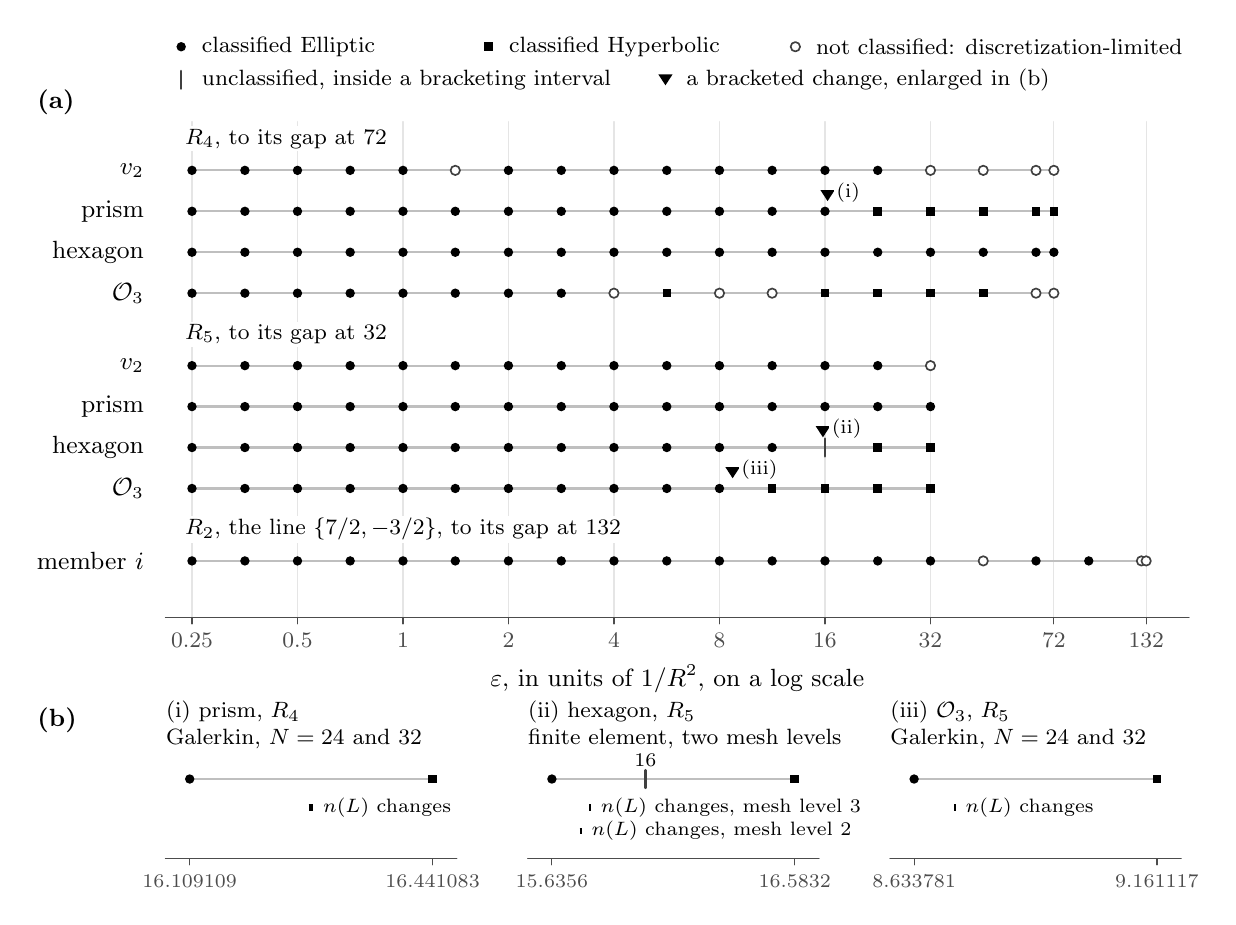
\begin{tikzpicture}[line cap=round, line join=round]
\draw[black!10] (0.337,-5.680) -- (0.337,0.620);
\draw[black!10] (1.677,-5.680) -- (1.677,0.620);
\draw[black!10] (3.017,-5.680) -- (3.017,0.620);
\draw[black!10] (4.356,-5.680) -- (4.356,0.620);
\draw[black!10] (5.696,-5.680) -- (5.696,0.620);
\draw[black!10] (7.036,-5.680) -- (7.036,0.620);
\draw[black!10] (8.376,-5.680) -- (8.376,0.620);
\draw[black!10] (9.716,-5.680) -- (9.716,0.620);
\draw[black!10] (11.283,-5.680) -- (11.283,0.620);
\draw[black!10] (12.455,-5.680) -- (12.455,0.620);
\node[font=\footnotesize, anchor=west, fill=white, inner sep=1pt] at (0.207,0.400) {$R_4$, to its gap at 72};
\node[font=\small, anchor=east] at (-0.15,0.000) {$v_2$};
\node[font=\small, anchor=east] at (-0.15,-0.520) {prism};
\node[font=\small, anchor=east] at (-0.15,-1.040) {hexagon};
\node[font=\small, anchor=east] at (-0.15,-1.560) {$\mathcal{O}_3$};
\node[font=\footnotesize, anchor=west, fill=white, inner sep=1pt] at (0.207,-2.080) {$R_5$, to its gap at 32};
\node[font=\small, anchor=east] at (-0.15,-2.480) {$v_2$};
\node[font=\small, anchor=east] at (-0.15,-3.000) {prism};
\node[font=\small, anchor=east] at (-0.15,-3.520) {hexagon};
\node[font=\small, anchor=east] at (-0.15,-4.040) {$\mathcal{O}_3$};
\node[font=\footnotesize, anchor=west, fill=white, inner sep=1pt] at (0.207,-4.560) {$R_2$, the line $\{7/2, -3/2\}$, to its gap at 132};
\node[font=\small, anchor=east] at (-0.15,-4.960) {member $i$};
\draw[black!25, line width=0.8pt] (0.337,0.000) -- (11.283,0.000);
\draw[black!25, line width=0.8pt] (0.337,-1.560) -- (11.283,-1.560);
\draw[black!25, line width=0.8pt] (0.337,-2.480) -- (9.716,-2.480);
\draw[black!25, line width=0.8pt] (0.337,-4.040) -- (9.716,-4.040);
\draw[black!25, line width=0.8pt] (0.337,-0.520) -- (11.283,-0.520);
\draw[black!25, line width=0.8pt] (0.337,-3.000) -- (9.716,-3.000);
\draw[black!25, line width=0.8pt] (0.337,-1.040) -- (11.283,-1.040);
\draw[black!25, line width=0.8pt] (0.337,-3.520) -- (9.716,-3.520);
\draw[black!25, line width=0.8pt] (0.337,-4.960) -- (12.455,-4.960);
\fill (0.337,0.000) circle (1.7pt);
\fill (1.009,0.000) circle (1.7pt);
\fill (1.677,0.000) circle (1.7pt);
\fill (2.346,0.000) circle (1.7pt);
\fill (3.017,0.000) circle (1.7pt);
\draw[black!75, fill=white, line width=0.6pt] (3.681,0.000) circle (1.7pt);
\fill (4.356,0.000) circle (1.7pt);
\fill (5.027,0.000) circle (1.7pt);
\fill (5.696,0.000) circle (1.7pt);
\fill (6.367,0.000) circle (1.7pt);
\fill (7.036,0.000) circle (1.7pt);
\fill (7.705,0.000) circle (1.7pt);
\fill (8.376,0.000) circle (1.7pt);
\fill (9.046,0.000) circle (1.7pt);
\draw[black!75, fill=white, line width=0.6pt] (9.716,0.000) circle (1.7pt);
\draw[black!75, fill=white, line width=0.6pt] (10.386,0.000) circle (1.7pt);
\draw[black!75, fill=white, line width=0.6pt] (11.056,0.000) circle (1.7pt);
\draw[black!75, fill=white, line width=0.6pt] (11.283,0.000) circle (1.7pt);
\fill (0.337,-1.560) circle (1.7pt);
\fill (1.009,-1.560) circle (1.7pt);
\fill (1.677,-1.560) circle (1.7pt);
\fill (2.346,-1.560) circle (1.7pt);
\fill (3.017,-1.560) circle (1.7pt);
\fill (3.681,-1.560) circle (1.7pt);
\fill (4.356,-1.560) circle (1.7pt);
\fill (5.027,-1.560) circle (1.7pt);
\draw[black!75, fill=white, line width=0.6pt] (5.696,-1.560) circle (1.7pt);
\fill ([shift={(-1.55pt,-1.55pt)}]6.367,-1.560) rectangle ++(3.1pt,3.1pt);
\draw[black!75, fill=white, line width=0.6pt] (7.036,-1.560) circle (1.7pt);
\draw[black!75, fill=white, line width=0.6pt] (7.705,-1.560) circle (1.7pt);
\fill ([shift={(-1.55pt,-1.55pt)}]8.376,-1.560) rectangle ++(3.1pt,3.1pt);
\fill ([shift={(-1.55pt,-1.55pt)}]9.046,-1.560) rectangle ++(3.1pt,3.1pt);
\fill ([shift={(-1.55pt,-1.55pt)}]9.716,-1.560) rectangle ++(3.1pt,3.1pt);
\fill ([shift={(-1.55pt,-1.55pt)}]10.386,-1.560) rectangle ++(3.1pt,3.1pt);
\draw[black!75, fill=white, line width=0.6pt] (11.056,-1.560) circle (1.7pt);
\draw[black!75, fill=white, line width=0.6pt] (11.283,-1.560) circle (1.7pt);
\fill (0.337,-2.480) circle (1.7pt);
\fill (1.009,-2.480) circle (1.7pt);
\fill (1.677,-2.480) circle (1.7pt);
\fill (2.346,-2.480) circle (1.7pt);
\fill (3.017,-2.480) circle (1.7pt);
\fill (3.681,-2.480) circle (1.7pt);
\fill (4.356,-2.480) circle (1.7pt);
\fill (5.027,-2.480) circle (1.7pt);
\fill (5.696,-2.480) circle (1.7pt);
\fill (6.367,-2.480) circle (1.7pt);
\fill (7.036,-2.480) circle (1.7pt);
\fill (7.705,-2.480) circle (1.7pt);
\fill (8.376,-2.480) circle (1.7pt);
\fill (9.046,-2.480) circle (1.7pt);
\draw[black!75, fill=white, line width=0.6pt] (9.716,-2.480) circle (1.7pt);
\fill (0.337,-4.040) circle (1.7pt);
\fill (1.009,-4.040) circle (1.7pt);
\fill (1.677,-4.040) circle (1.7pt);
\fill (2.346,-4.040) circle (1.7pt);
\fill (3.017,-4.040) circle (1.7pt);
\fill (3.681,-4.040) circle (1.7pt);
\fill (4.356,-4.040) circle (1.7pt);
\fill (5.027,-4.040) circle (1.7pt);
\fill (5.696,-4.040) circle (1.7pt);
\fill (6.367,-4.040) circle (1.7pt);
\fill (7.036,-4.040) circle (1.7pt);
\fill ([shift={(-1.55pt,-1.55pt)}]7.705,-4.040) rectangle ++(3.1pt,3.1pt);
\fill ([shift={(-1.55pt,-1.55pt)}]8.376,-4.040) rectangle ++(3.1pt,3.1pt);
\fill ([shift={(-1.55pt,-1.55pt)}]9.046,-4.040) rectangle ++(3.1pt,3.1pt);
\fill ([shift={(-1.55pt,-1.55pt)}]9.716,-4.040) rectangle ++(3.1pt,3.1pt);
\fill (7.203,-3.910) -- ++(-2.6pt,4pt) -- ++(5.2pt,0) -- cycle;
\node[font=\scriptsize, anchor=west, fill=white, inner sep=1pt] at (7.273,-3.800) {(iii)};
\fill (0.337,-0.520) circle (1.7pt);
\fill (1.009,-0.520) circle (1.7pt);
\fill (1.677,-0.520) circle (1.7pt);
\fill (2.346,-0.520) circle (1.7pt);
\fill (3.017,-0.520) circle (1.7pt);
\fill (3.681,-0.520) circle (1.7pt);
\fill (4.356,-0.520) circle (1.7pt);
\fill (5.027,-0.520) circle (1.7pt);
\fill (5.696,-0.520) circle (1.7pt);
\fill (6.367,-0.520) circle (1.7pt);
\fill (7.036,-0.520) circle (1.7pt);
\fill (7.705,-0.520) circle (1.7pt);
\fill (8.376,-0.520) circle (1.7pt);
\fill ([shift={(-1.55pt,-1.55pt)}]9.046,-0.520) rectangle ++(3.1pt,3.1pt);
\fill ([shift={(-1.55pt,-1.55pt)}]9.716,-0.520) rectangle ++(3.1pt,3.1pt);
\fill ([shift={(-1.55pt,-1.55pt)}]10.386,-0.520) rectangle ++(3.1pt,3.1pt);
\fill ([shift={(-1.55pt,-1.55pt)}]11.056,-0.520) rectangle ++(3.1pt,3.1pt);
\fill ([shift={(-1.55pt,-1.55pt)}]11.283,-0.520) rectangle ++(3.1pt,3.1pt);
\fill (8.409,-0.390) -- ++(-2.6pt,4pt) -- ++(5.2pt,0) -- cycle;
\node[font=\scriptsize, anchor=west, fill=white, inner sep=1pt] at (8.479,-0.280) {(i)};
\fill (0.337,-3.000) circle (1.7pt);
\fill (1.009,-3.000) circle (1.7pt);
\fill (1.677,-3.000) circle (1.7pt);
\fill (2.346,-3.000) circle (1.7pt);
\fill (3.017,-3.000) circle (1.7pt);
\fill (3.681,-3.000) circle (1.7pt);
\fill (4.356,-3.000) circle (1.7pt);
\fill (5.027,-3.000) circle (1.7pt);
\fill (5.696,-3.000) circle (1.7pt);
\fill (6.367,-3.000) circle (1.7pt);
\fill (7.036,-3.000) circle (1.7pt);
\fill (7.705,-3.000) circle (1.7pt);
\fill (8.376,-3.000) circle (1.7pt);
\fill (9.046,-3.000) circle (1.7pt);
\fill (9.716,-3.000) circle (1.7pt);
\fill (0.337,-1.040) circle (1.7pt);
\fill (1.009,-1.040) circle (1.7pt);
\fill (1.677,-1.040) circle (1.7pt);
\fill (2.346,-1.040) circle (1.7pt);
\fill (3.017,-1.040) circle (1.7pt);
\fill (3.681,-1.040) circle (1.7pt);
\fill (4.356,-1.040) circle (1.7pt);
\fill (5.027,-1.040) circle (1.7pt);
\fill (5.696,-1.040) circle (1.7pt);
\fill (6.367,-1.040) circle (1.7pt);
\fill (7.036,-1.040) circle (1.7pt);
\fill (7.705,-1.040) circle (1.7pt);
\fill (8.376,-1.040) circle (1.7pt);
\fill (9.046,-1.040) circle (1.7pt);
\fill (9.716,-1.040) circle (1.7pt);
\fill (10.386,-1.040) circle (1.7pt);
\fill (11.056,-1.040) circle (1.7pt);
\fill (11.283,-1.040) circle (1.7pt);
\fill (0.337,-3.520) circle (1.7pt);
\fill (1.009,-3.520) circle (1.7pt);
\fill (1.677,-3.520) circle (1.7pt);
\fill (2.346,-3.520) circle (1.7pt);
\fill (3.017,-3.520) circle (1.7pt);
\fill (3.681,-3.520) circle (1.7pt);
\fill (4.356,-3.520) circle (1.7pt);
\fill (5.027,-3.520) circle (1.7pt);
\fill (5.696,-3.520) circle (1.7pt);
\fill (6.367,-3.520) circle (1.7pt);
\fill (7.036,-3.520) circle (1.7pt);
\fill (7.705,-3.520) circle (1.7pt);
\draw[black!75, line width=0.9pt] ([yshift=-3.2pt]8.376,-3.520) -- ([yshift=3.2pt]8.376,-3.520);
\fill ([shift={(-1.55pt,-1.55pt)}]9.046,-3.520) rectangle ++(3.1pt,3.1pt);
\fill ([shift={(-1.55pt,-1.55pt)}]9.716,-3.520) rectangle ++(3.1pt,3.1pt);
\fill (8.350,-3.390) -- ++(-2.6pt,4pt) -- ++(5.2pt,0) -- cycle;
\node[font=\scriptsize, anchor=west, fill=white, inner sep=1pt] at (8.420,-3.280) {(ii)};
\fill (0.337,-4.960) circle (1.7pt);
\fill (1.009,-4.960) circle (1.7pt);
\fill (1.677,-4.960) circle (1.7pt);
\fill (2.346,-4.960) circle (1.7pt);
\fill (3.017,-4.960) circle (1.7pt);
\fill (3.681,-4.960) circle (1.7pt);
\fill (4.356,-4.960) circle (1.7pt);
\fill (5.027,-4.960) circle (1.7pt);
\fill (5.696,-4.960) circle (1.7pt);
\fill (6.367,-4.960) circle (1.7pt);
\fill (7.036,-4.960) circle (1.7pt);
\fill (7.705,-4.960) circle (1.7pt);
\fill (8.376,-4.960) circle (1.7pt);
\fill (9.046,-4.960) circle (1.7pt);
\fill (9.716,-4.960) circle (1.7pt);
\draw[black!75, fill=white, line width=0.6pt] (10.386,-4.960) circle (1.7pt);
\fill (11.056,-4.960) circle (1.7pt);
\fill (11.726,-4.960) circle (1.7pt);
\draw[black!75, fill=white, line width=0.6pt] (12.395,-4.960) circle (1.7pt);
\draw[black!75, fill=white, line width=0.6pt] (12.455,-4.960) circle (1.7pt);
\draw[black!70] (0.000,-5.680) -- (13.000,-5.680);
\draw[black!70] (0.337,-5.680) -- ++(0,-0.08) node[below, font=\footnotesize] {0.25};
\draw[black!70] (1.677,-5.680) -- ++(0,-0.08) node[below, font=\footnotesize] {0.5};
\draw[black!70] (3.017,-5.680) -- ++(0,-0.08) node[below, font=\footnotesize] {1};
\draw[black!70] (4.356,-5.680) -- ++(0,-0.08) node[below, font=\footnotesize] {2};
\draw[black!70] (5.696,-5.680) -- ++(0,-0.08) node[below, font=\footnotesize] {4};
\draw[black!70] (7.036,-5.680) -- ++(0,-0.08) node[below, font=\footnotesize] {8};
\draw[black!70] (8.376,-5.680) -- ++(0,-0.08) node[below, font=\footnotesize] {16};
\draw[black!70] (9.716,-5.680) -- ++(0,-0.08) node[below, font=\footnotesize] {32};
\draw[black!70] (11.283,-5.680) -- ++(0,-0.08) node[below, font=\footnotesize] {72};
\draw[black!70] (12.455,-5.680) -- ++(0,-0.08) node[below, font=\footnotesize] {132};
\node[font=\small] at (6.500,-6.460) {$\varepsilon$, in units of $1/R^2$, on a log scale};
\fill (0.200,1.570) circle (1.7pt);
\node[font=\footnotesize, anchor=west] at (0.340,1.570) {classified Elliptic};
\fill ([shift={(-1.55pt,-1.55pt)}]4.100,1.570) rectangle ++(3.1pt,3.1pt);
\node[font=\footnotesize, anchor=west] at (4.240,1.570) {classified Hyperbolic};
\draw[black!75, fill=white, line width=0.6pt] (8.000,1.570) circle (1.7pt);
\node[font=\footnotesize, anchor=west] at (8.140,1.570) {not classified: discretization-limited};
\draw[black!75, line width=0.9pt] ([yshift=-3.2pt]0.200,1.150) -- ([yshift=3.2pt]0.200,1.150);
\node[font=\footnotesize, anchor=west] at (0.340,1.150) {unclassified, inside a bracketing interval};
\fill (6.350,1.080) -- ++(-2.6pt,4pt) -- ++(5.2pt,0) -- cycle;
\node[font=\footnotesize, anchor=west] at (6.490,1.150) {a bracketed change, enlarged in (b)};
\node[font=\small\bfseries, anchor=west] at (-1.75,0.870) {(a)};
\node[font=\small\bfseries, anchor=west] at (-1.75,-6.980) {(b)};
\node[font=\footnotesize, anchor=south west, align=left, inner sep=0pt] at (0.000,-7.350) {(i) prism, $R_4$\\ Galerkin, $N = 24$ and 32};
\draw[black!25, line width=0.8pt] (0.308,-7.730) -- (3.392,-7.730);
\fill (0.308,-7.730) circle (1.7pt);
\fill ([shift={(-1.55pt,-1.55pt)}]3.392,-7.730) rectangle ++(3.1pt,3.1pt);
\draw[line width=2.4pt, line cap=butt] (1.8196,-8.090) -- (1.8798,-8.090);
\node[font=\scriptsize, anchor=west, inner sep=1pt] at (1.960,-8.090) {$n(L)$ changes};
\draw[black!70] (0.000,-8.740) -- (3.700,-8.740);
\draw[black!70] (0.308,-8.740) -- ++(0,-0.08) node[below, font=\scriptsize] {16.109109};
\draw[black!70] (3.392,-8.740) -- ++(0,-0.08) node[below, font=\scriptsize] {16.441083};
\node[font=\footnotesize, anchor=south west, align=left, inner sep=0pt] at (4.600,-7.350) {(ii) hexagon, $R_5$\\ finite element, two mesh levels};
\draw[black!25, line width=0.8pt] (4.908,-7.730) -- (7.992,-7.730);
\fill (4.908,-7.730) circle (1.7pt);
\fill ([shift={(-1.55pt,-1.55pt)}]7.992,-7.730) rectangle ++(3.1pt,3.1pt);
\draw[black!75, line width=0.9pt] ([yshift=-3.2pt]6.094,-7.730) -- ([yshift=3.2pt]6.094,-7.730);
\node[font=\scriptsize, above, inner sep=2pt] at (6.094,-7.650) {16};
\draw[line width=2.4pt, line cap=butt] (5.3792,-8.090) -- (5.4091,-8.090);
\node[font=\scriptsize, anchor=west, inner sep=1pt] at (5.489,-8.090) {$n(L)$ changes, mesh level 3};
\draw[line width=2.4pt, line cap=butt] (5.2601,-8.390) -- (5.2900,-8.390);
\node[font=\scriptsize, anchor=west, inner sep=1pt] at (5.370,-8.390) {$n(L)$ changes, mesh level 2};
\draw[black!70] (4.600,-8.740) -- (8.300,-8.740);
\draw[black!70] (4.908,-8.740) -- ++(0,-0.08) node[below, font=\scriptsize] {15.6356};
\draw[black!70] (7.992,-8.740) -- ++(0,-0.08) node[below, font=\scriptsize] {16.5832};
\node[font=\footnotesize, anchor=south west, align=left, inner sep=0pt] at (9.200,-7.350) {(iii) $\mathcal{O}_3$, $R_5$\\ Galerkin, $N = 24$ and 32};
\draw[black!25, line width=0.8pt] (9.508,-7.730) -- (12.592,-7.730);
\fill (9.508,-7.730) circle (1.7pt);
\fill ([shift={(-1.55pt,-1.55pt)}]12.592,-7.730) rectangle ++(3.1pt,3.1pt);
\draw[line width=2.4pt, line cap=butt] (10.0182,-8.090) -- (10.0410,-8.090);
\node[font=\scriptsize, anchor=west, inner sep=1pt] at (10.121,-8.090) {$n(L)$ changes};
\draw[black!70] (9.200,-8.740) -- (12.900,-8.740);
\draw[black!70] (9.508,-8.740) -- ++(0,-0.08) node[below, font=\scriptsize] {8.633781};
\draw[black!70] (12.592,-8.740) -- ++(0,-0.08) node[below, font=\scriptsize] {9.161117};
\end{tikzpicture}
\end{document}
